\documentclass[twoside,openright,a4paper,11pt,french]{article}
\usepackage[utf8]{inputenc}
\usepackage[french]{babel}
\usepackage[T1]{fontenc}
\usepackage{emptypage}
\usepackage{amsmath}

% Utilisation d'url
\usepackage{url}
\urlstyle{sf}

% Utilisation d'images, stockées dans le répertoire ./pics/
\usepackage{graphicx}
\graphicspath{pics/}

% Définition des marges
\usepackage{geometry}
\geometry{
  left=25mm,
  right=25mm,
  top=25mm,
  bottom=25mm,
  foot=15mm
}
\usepackage{listings}
\usepackage{color}

\definecolor{gray}{rgb}{0.8,0.8,0.8}

\begin{document}

\pagestyle{plain}
\setlength{\parindent}{0pt}
% La page de garde
\thispagestyle{empty}

\begin{center}
       \noindent
       
\includegraphics[height=2.5cm]{./pics/uds.eps}       
       
       \vfill\vfill

    {\large \textsc{Licence 3 de Sciences, mention Informatique}}

    \bigskip\bigskip

    {\large \textsc{Intelligence Artificielle}}

    \vfill\vfill

% Titre du document
    {\huge \sc
      \begin{center} 
        Rapport sur le projet: \\
        Perceptron et perceptron multi-couchers avec Neuroph
      \end{center}}

    \vfill\vfill

    {\large Présenté par}

\medskip

% Identité des auteurs
    {\large Victor \textsc{Constans}}\\
    {\large Luigi  \textsc{Coniglio}}\\
\bigskip

\end{center}



% La table des matières
\parskip=0pt
\tableofcontents


\vspace{5cm}

%Start content

\section{Fonctions booléennes}

Dans cette premiere section de ce rapport on se propose
de implementer des fonctions booléennes a l'aide des reseaux
de neurones. 

\subsection{"Et" logique}

En matematique la conjonction logique $\land$ est un
connecteur logique que, etant donne deux propositions $A$ et $B$
forme une nouvelle propositions $A \land B$ qui est vrai seulement
si $A$ et $B$ sont vraies.

\begin{table}[h]
  \centering
  \begin{tabular}{| c | c | c |}
    \hline
    \textbf{$A$} & \textbf{$B$} & \textbf{$A \land B$}\\
    \hline
    0 & 0  & 0 \\
    \hline
    0 & 1  & 0 \\
    \hline
    1 & 0  & 0 \\
    \hline
    1 & 1  & 1 \\
    \hline
  \end{tabular}
  \caption{Table de verite de $A \land B$}
  \label{tab:et}
\end{table}




\subsubsection{Un perceptron pour $\land$} 

Est it possible d'utiliser un perceptron pour apprendre la fonction logique
"et"? Bien sur, en effet meme un perceptron mono couche est sufficent pour
obtenir cet resultat.\\

Le perceptron peut etre utilise comme un classifieur linéaire, cad. l'algorithme du
perceptron perment de reconnaitre et donc classifier des donnes (ou points)
linearement separables.\\

Un ensemble de points dans le plan caracterise par deux sous-classes disjointes
de points, est dit linearement separable si il existe une droite qui separe
completement les deux sous-classes.\\

Dans trois dimension un ensemble est linearement separable si il existe un plan
qui separe les deux classes. Dans quatre ou plus dimensions on ne parlera plus de
plan mais de hyperplan.


\begin{figure}[h]
\centering
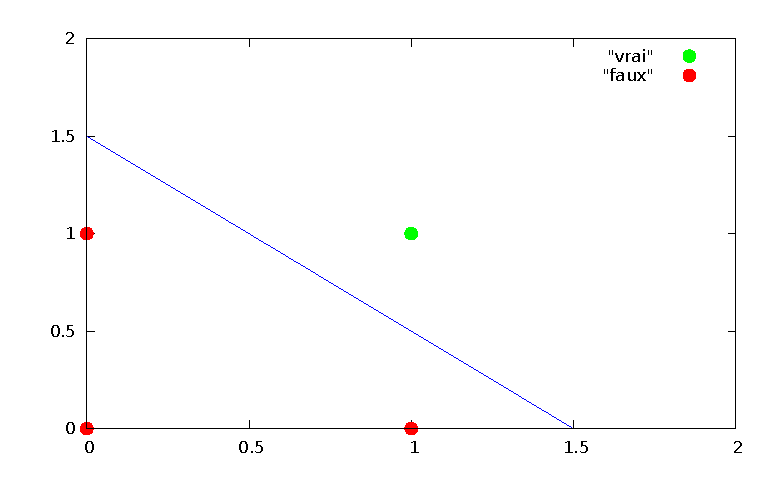
\includegraphics[width=10cm]{./pics/and/and.eps}
\caption{La fonction logique "et" est linearement separable}
\label{fig:and}
\end{figure}


Comme montre la figure \ref{fig:and} la fonction "et" est bien linearement
separable. Etant donne que tout ensemble linéairement séparable peut être
discriminé par un perceptron on est sur de pouvoir trouver un perceptron qui
engendre la fonction booléenne $\land$.\\

Le perceptron cree avec Neuroph que on utilisera pour cette fonction 
est vraiment tres simple et est inllustre dans la figure \ref{fig:per_and}.
Le data set pour l'apprentissage contiens les meme valeurs de la table
\ref{tab:et}.

\begin{figure}[h]
\centering
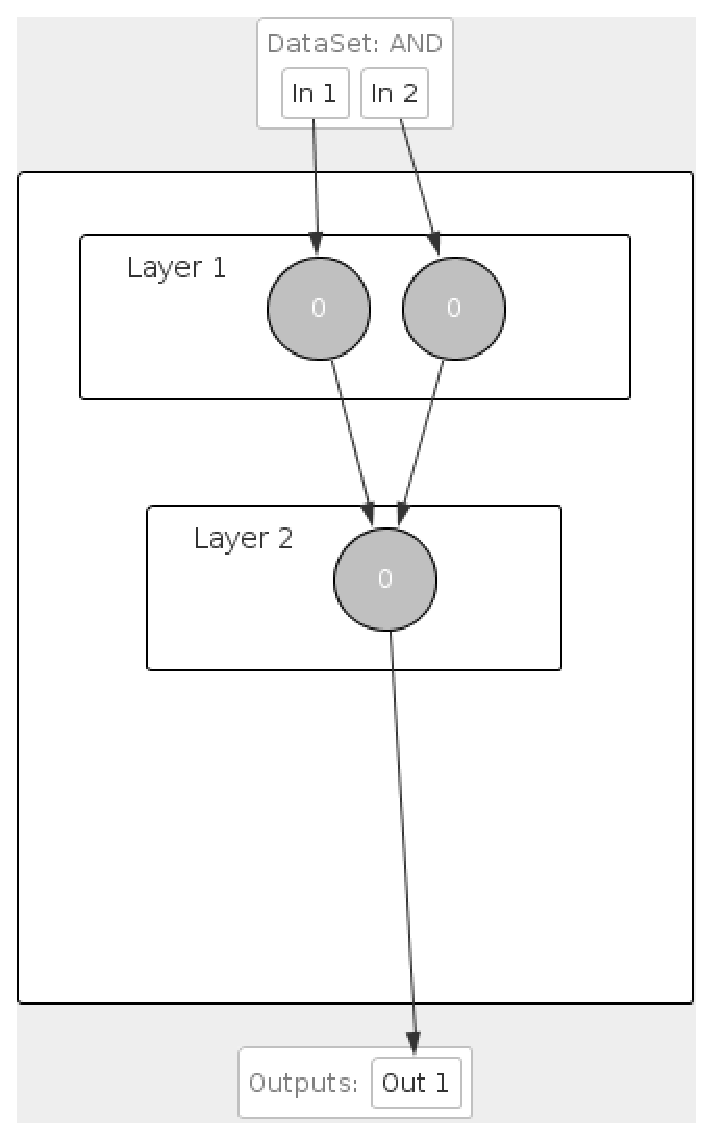
\includegraphics[width=4.5cm,height=7cm]{./pics/perc_and.eps}
\caption{Perceptron pour la fonction "et"}
\label{fig:per_and}
\end{figure}

Pendant l'entrainement du perceptron (dont les poids ont ete initialize avant
aleatoireament) avec des avec un taux d'apprentissage de 0.2 (valeur par
default) on obtient une courbe d'apprentissage qui converge toujours a
zero. La forme de celle-ci dependra essentialement des valeurs initiales des
poids. 


\begin{figure}[h]
\centering
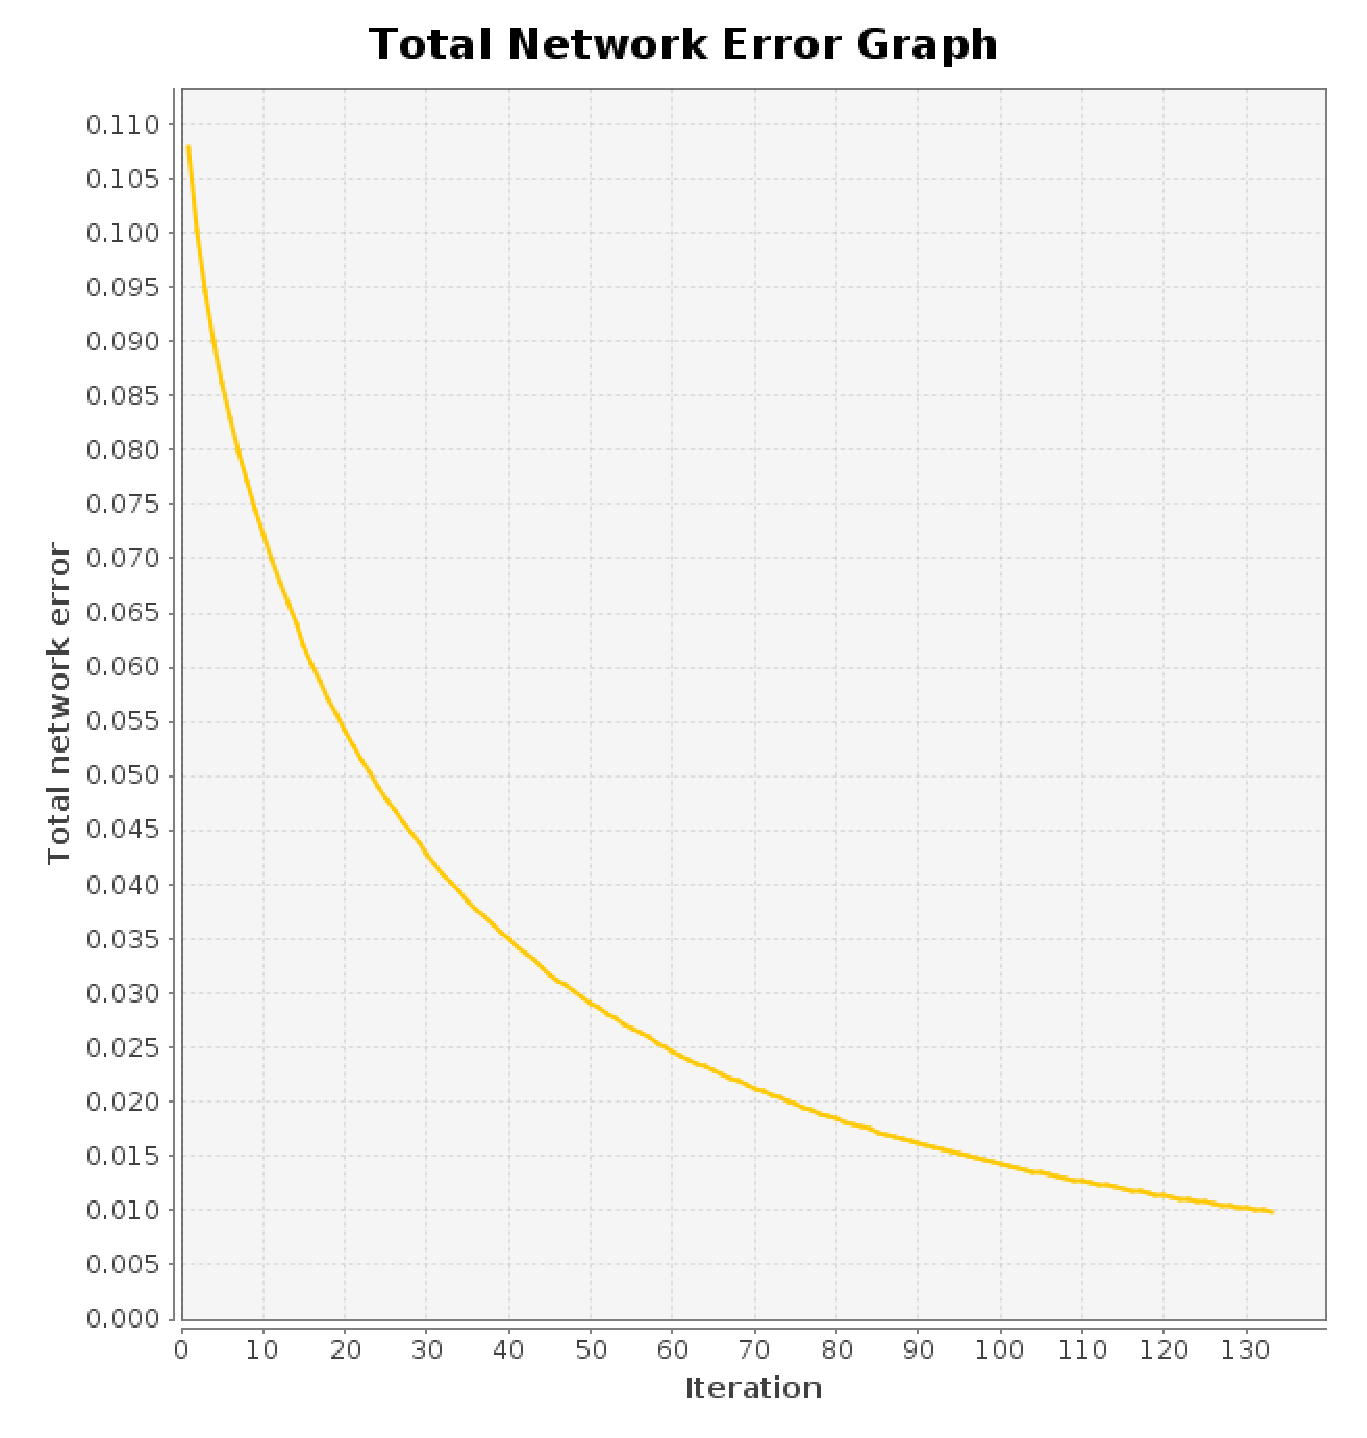
\includegraphics[width=12cm,height=9cm]{./pics/and_error1.eps}
\caption{Exemple de courbe d'apprentissage pour la fonction "et"}
\label{fig:anderr}
\end{figure}

La figure \ref{fig:anderr} montre un exemple de courbe d'apprentissage
obtenu avec les valeurs susmentionne.\\

L'apprentissage peut etre pense comme le processus pendat le quelle la
reseau de neurons cherche de s'approcher le plus possible au plus petit
taux d'erreur.\\

En effet, la meilleure configuration (valeurs des poids, biais, etc.) pour
notre reseau de neurons corresponde au point de minimum globale de la fonction
$E$ qui associe a toute configuration de notre reseau de neurons un cout $C$.\\

$E$ mesure la difference entre le valeur attendu et celui produit et est
souvent calcule comme etant $E(y,y') = \tfrac{1}{2} \lVert y-y'\rVert^2$ ou $y$ est
le valeur attendu et $y'$ est le valeur produit par la reseau.
Mais pourquoi pas plus simplement $\lVert y-y'\rVert$? 
En effet, la choix d'utiliser une fonction quadratique n'est pas casuelle. 
Un des problemes plus importantes dans l'apprentissage supervisee d'une reseau
de neurones qui se base sur l'algorithme du gradient (gradient descent) est
celui pose par les points de minimum locales de $E$. Le fait que $E$ soit
quadratique permet d'exploiter la convexite des fonctions quadratique pour
minimizer ce probleme. Le $\tfrac{1}{2}$ permet de simplifier la fonction lors
de sa derivation.\\

Comme attendu, dans notre cas le perceptron n'a aucun probleme a trouver le
minimum globale de $E$ mais dans ce premiere exemple on se contente d'entrainer la
reseau de neurons jusq'a obtenir un taux d'erreur moyen de seulement 1\%. La
figure \ref{fig:andtest1} montre les resultat de l'entrainement:

\begin{figure}[h]
\centering
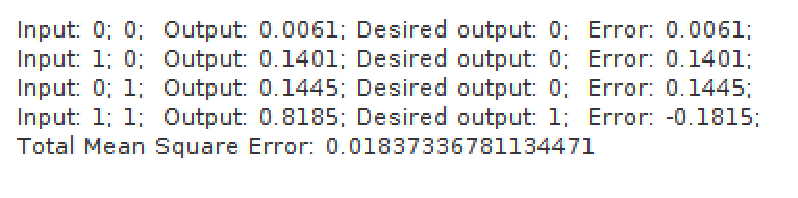
\includegraphics[width=7.3cm,height=2.3cm]{./pics/andtest1.eps}
\caption{Test d'erreur apres l'apprentissage de la fonction "et"}
\label{fig:andtest1}
\end{figure}

En utilisant la definition de $E$ on peut verifier que le cout
moyen est bien tres proche de $0.01$:

\begin{equation*}
  \begin{aligned}
  \tfrac{1}{4}\times(E(0,0.0061)+E(0,0.1401)+E(0,0.1445)+E(1,0.8185))\\
  = \tfrac{1}{4}\times(\tfrac{0.0061^2}{2}+\tfrac{0.1401^2}{2}+\tfrac{0.1445^2}{2}+\tfrac{0.1815^2}{2}) =
  0.009185965
  \end{aligned}
\end{equation*}

Le resultat obtenu est tres proche de celui souhaite, en effet il suffit de 
introduire une seuille pour obtenir un output qui soit un 0 ou un 1.
Dans Neuroph ca se traduit par utiliset la fonction d'activation step pour le
neuron d'output.


\begin{figure}[h]
\centering
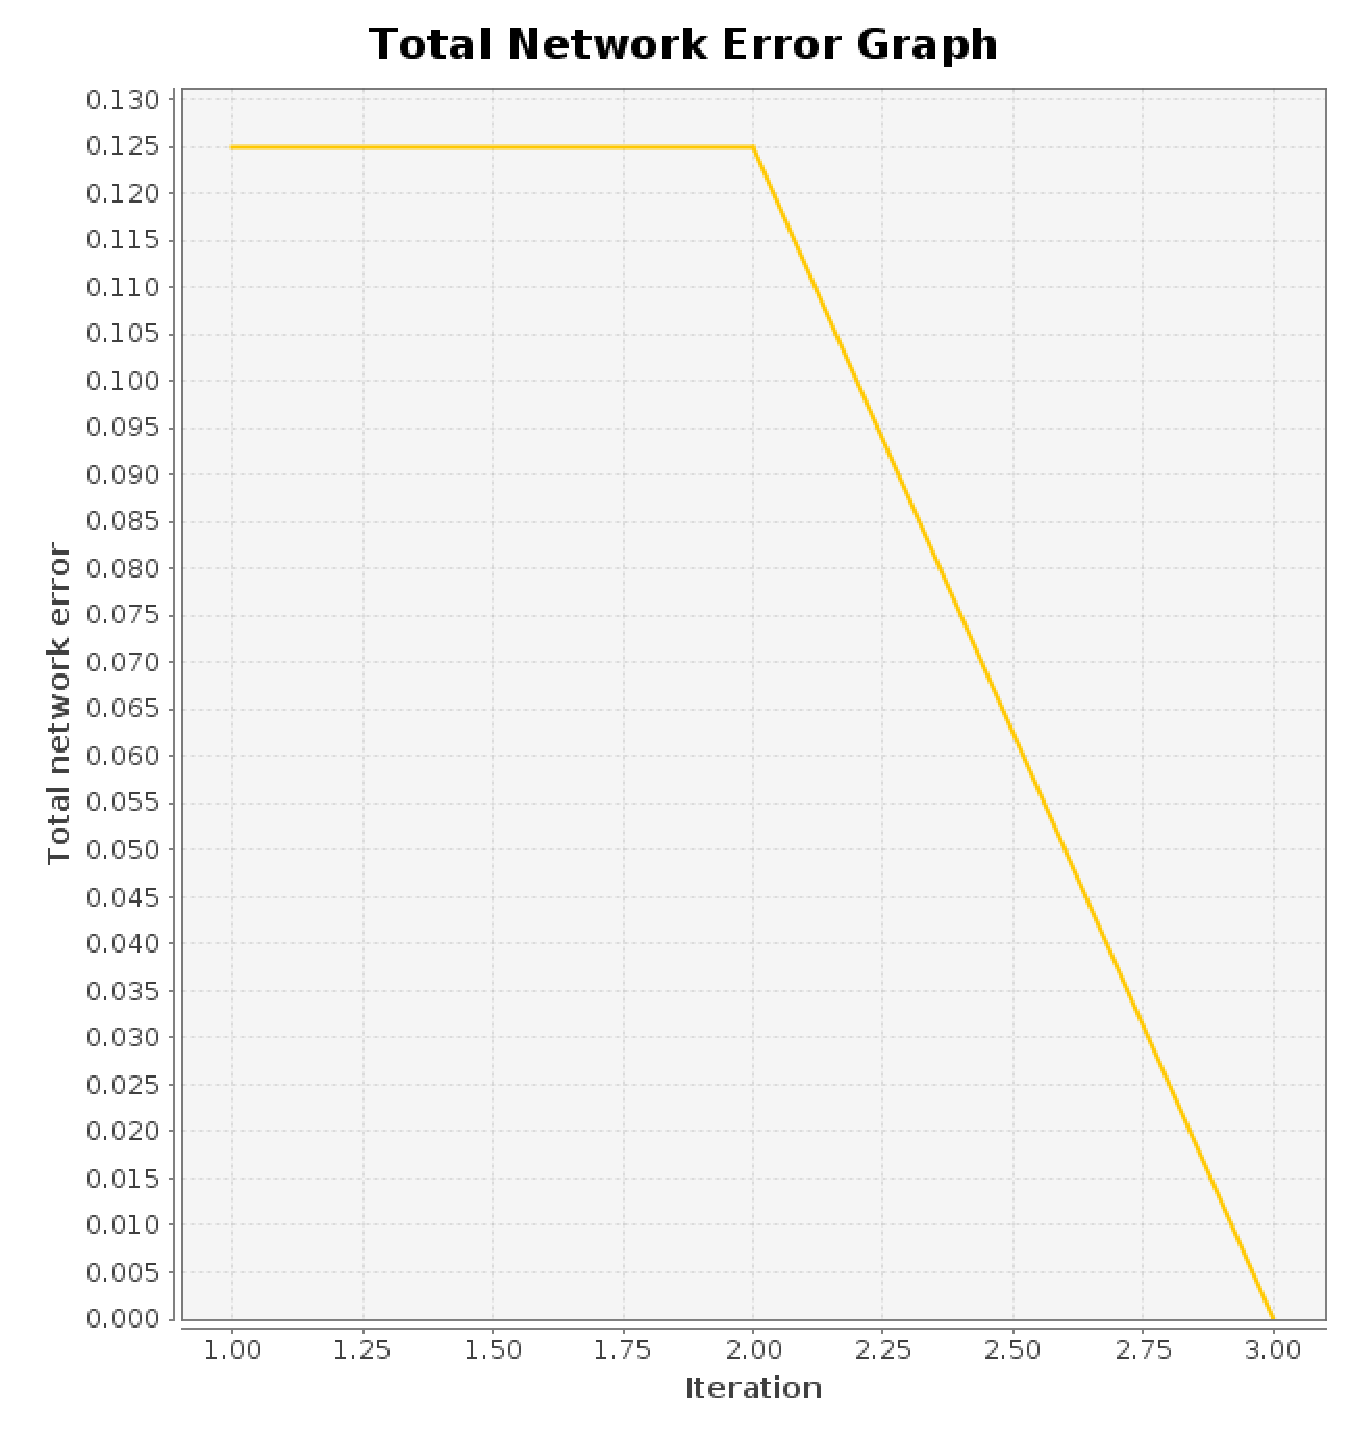
\includegraphics[width=12cm,height=9cm]{./pics/and_error2.eps}
\caption{Courbe d'apprentissage de "et" en utilisant la fonction step}
\label{fig:anderr}
\end{figure}



Cette technique nous perment d'obtenir une sortie parfaite qui ne presente
aucun taux d'erreur.



\begin{figure}[h]
\centering
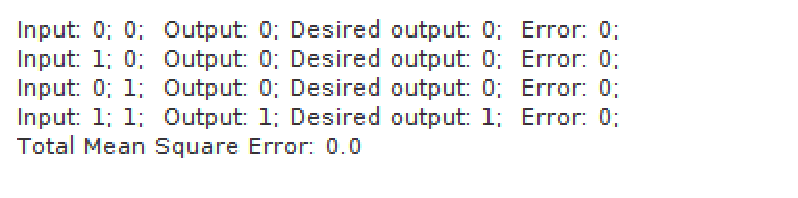
\includegraphics[width=7.3cm,height=2.3cm]{./pics/andtest2.eps}
\caption{Test d'erreur apres l'apprentissage de la fonction "et"}
\label{fig:andtest2}
\end{figure}


\subsubsection{Differents pas d'apprentissage}

Le pas d'apprentissage determine la vitesse (pas) avec la quelle notre reseau
cherche a s'approcher au point d'erreur minimum. 
A chaque epoque ({\it batch learning}) ou a chaque iteration ({\it incremental
learning}) les poids de la reseau sont mise a jour en utilisant une combinaison du
pas d'apprentissage et le gradient $\nabla E$ qui indique la direction du taux
d'accroissement le plus élevé de $E$ et sa pente.\\

Le pas d'apprentissage joue un role tres importante dans la recherche du
minimum globale d'une fonction. 
Si un pas d'apprentissage trop grand risque de ne pas atteindre le minimum globale
un pas trop petit augment le temps necessaire a entrainer le reseau et risque de
se bloquer dans un point de minimum locale.\\

Dans notre cas le changement du pas d'apprentissage n'a aucun effect que celui 
de changer la vitesse d'apprentissage.


\begin{figure}[h]
\centering
\includegraphics[width=12cm,height=9cm]{./pics/and_error3.eps}
\caption{Apprentissage fonction "et" avec un pas de 0.1}
\label{fig:anderr3}
\end{figure}

\begin{figure}[h]
\centering
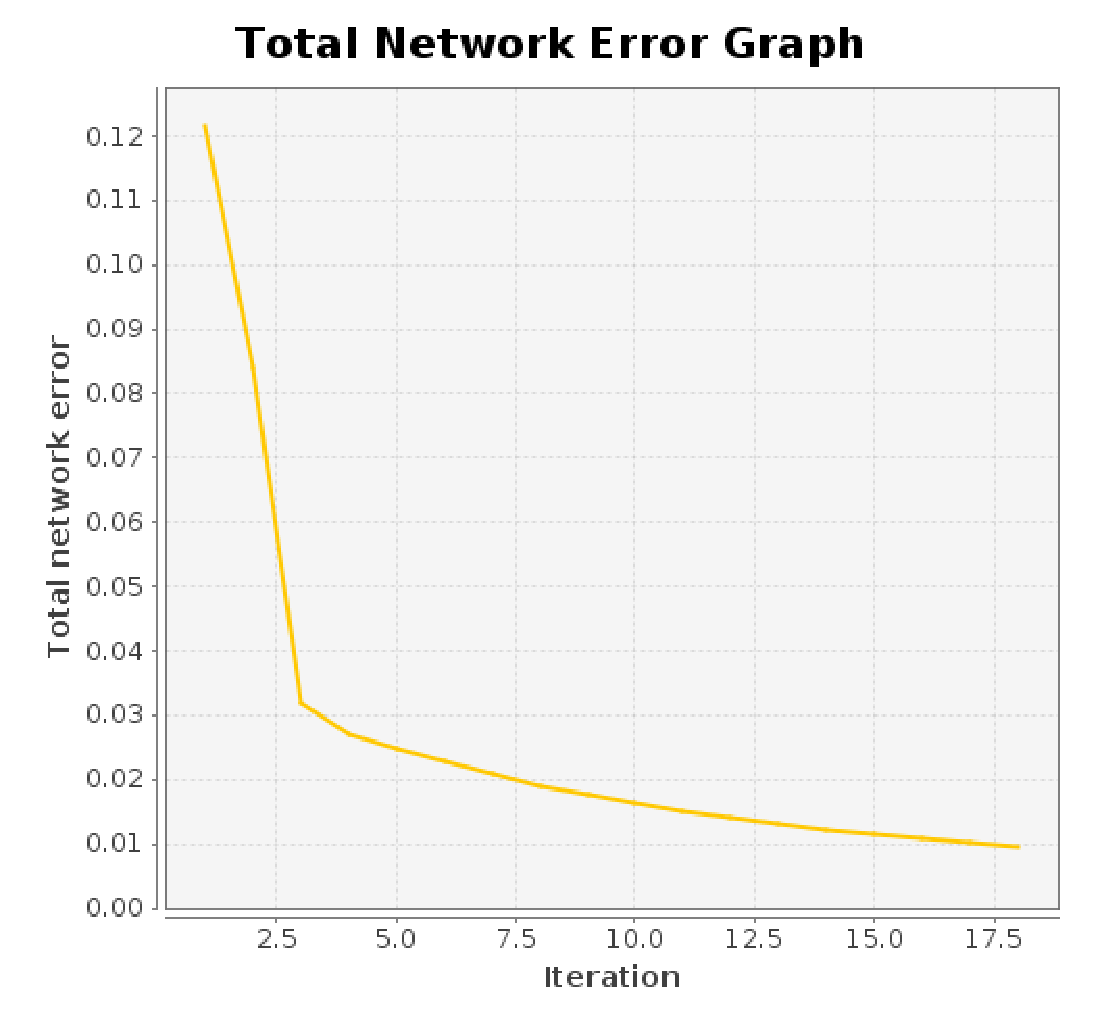
\includegraphics[width=12cm,height=9cm]{./pics/and_error4.eps}
\caption{Apprentissage fonction "et" avec un pas de 1}
\label{fig:anderr4}
\end{figure}

Avec un pas de 1 (figure \ref{fig:anderr4}) l'erreur totale du perceptron
tombe au-dessus de 0.01 apres seulement 17 iterations, par contre avec 
un pas de 0.1 le nombre d'iterations necessaires pour obtenir le meme
resultat monte a plus de 155 iterations (figure \ref{fig:anderr3}).

\subsection{Equivalence logique}
En matematique deux propositions sont dites equivalentes si l'un implique
l'autre: $a \Leftrightarrow b$. La table de verite de l'equivalence logique
est illustre par la table \ref{tab:eq}.


\begin{table}[h]
  \centering
  \begin{tabular}{| c | c | c |}
    \hline
    \textbf{$a$} & \textbf{$b$} & \textbf{$a \Leftrightarrow b$}\\
    \hline
    0 & 0  & 1 \\
    \hline
    0 & 1  & 0 \\
    \hline
    1 & 0  & 0 \\
    \hline
    1 & 1  & 1 \\
    \hline
  \end{tabular}
  \caption{Table de verite de $a \Leftrightarrow b$}
  \label{tab:eq}
\end{table}

\subsubsection{Un perceptron pour $\Leftrightarrow$}

\iffalse
% TODO %
1) En suivant l'exemple precedent proposer un perceptron mono couche pour
   l'equivalence logique 
    - Montrer la courbe d'apprentissage:
    - Expliquer pourquoi la courbe d'apprentissage ne converge pas
        --> Parceque l'eq. n'est pas linearement separable
    - Montrer que avec un pas d'apprentissage different le resultat
      ne change pas (essayer avec 0.1 et 1)
2) Proposer un perceptron multi-couches
    - Montrer que l'apprentissage converge
3) Montrer les resultats en changeant:
    - pas d'apprentissage
    - fonction d'activation
    - nombre de neurones
    - nombre de couches 
    ==> faire beaucoup de screenshots de Neuroph :)
        (ex. resultats des test, interface 
NB:
  - pas besoin de screenshot pour la courbe d'apprentissage
    on peut la sauvgarder directement
  - pour convertir un image au format eps (pour latex) il suffit
    simplement `convert image.truc image.eps` sur bash
  - si il y a besoin de generer des images avec gnuplot 
    je peut me n'occuper
\fi


\section{Apprentissage d'une fonction}
Pour l'apprentissage de la fonction carré nous avons décidé d'utiliser un perceptron
multi-couche car %TODO
Nous avons donc créé un perceptron avec une couche caché composé de %TODO 6 neurones.
Pour entrainer notre perceptron nous avons tout d'abord utilisé un data set contenant
les carrés pour de 1 jusqu'à 10. Pour avoir un data set compris entre 0 et 1 nous avons
normalisé notre data set.

\begin{table}[h]
  \centering
  \begin{tabular}{| c | c |}
    \hline
    \textbf{$a$} & \textbf{$b$} & \Leftrightarrow b$}\\
    \hline
    0.1 & 0.01 \\
    \hline
    0.2 & 0.04 \\
    \hline
    0.3 & 0.09 \\
    \hline
    0.4 & 0.16 \\
    \hline
    0.5 & 0.25 \\
    \hline
    0.6 & 0.36 \\
    \hline
    0.7 & 0.49 \\
    \hline
    0.8 & 0.64 \\
    \hline
    0.9 & 0.81 \\
    \hline
    1.0 & 1.0 \\
    \hline
  \end{tabular}
  \caption{Data set de la fonction carré \Leftrightarrow b$}
  \label{tab:eq}
\end{table}

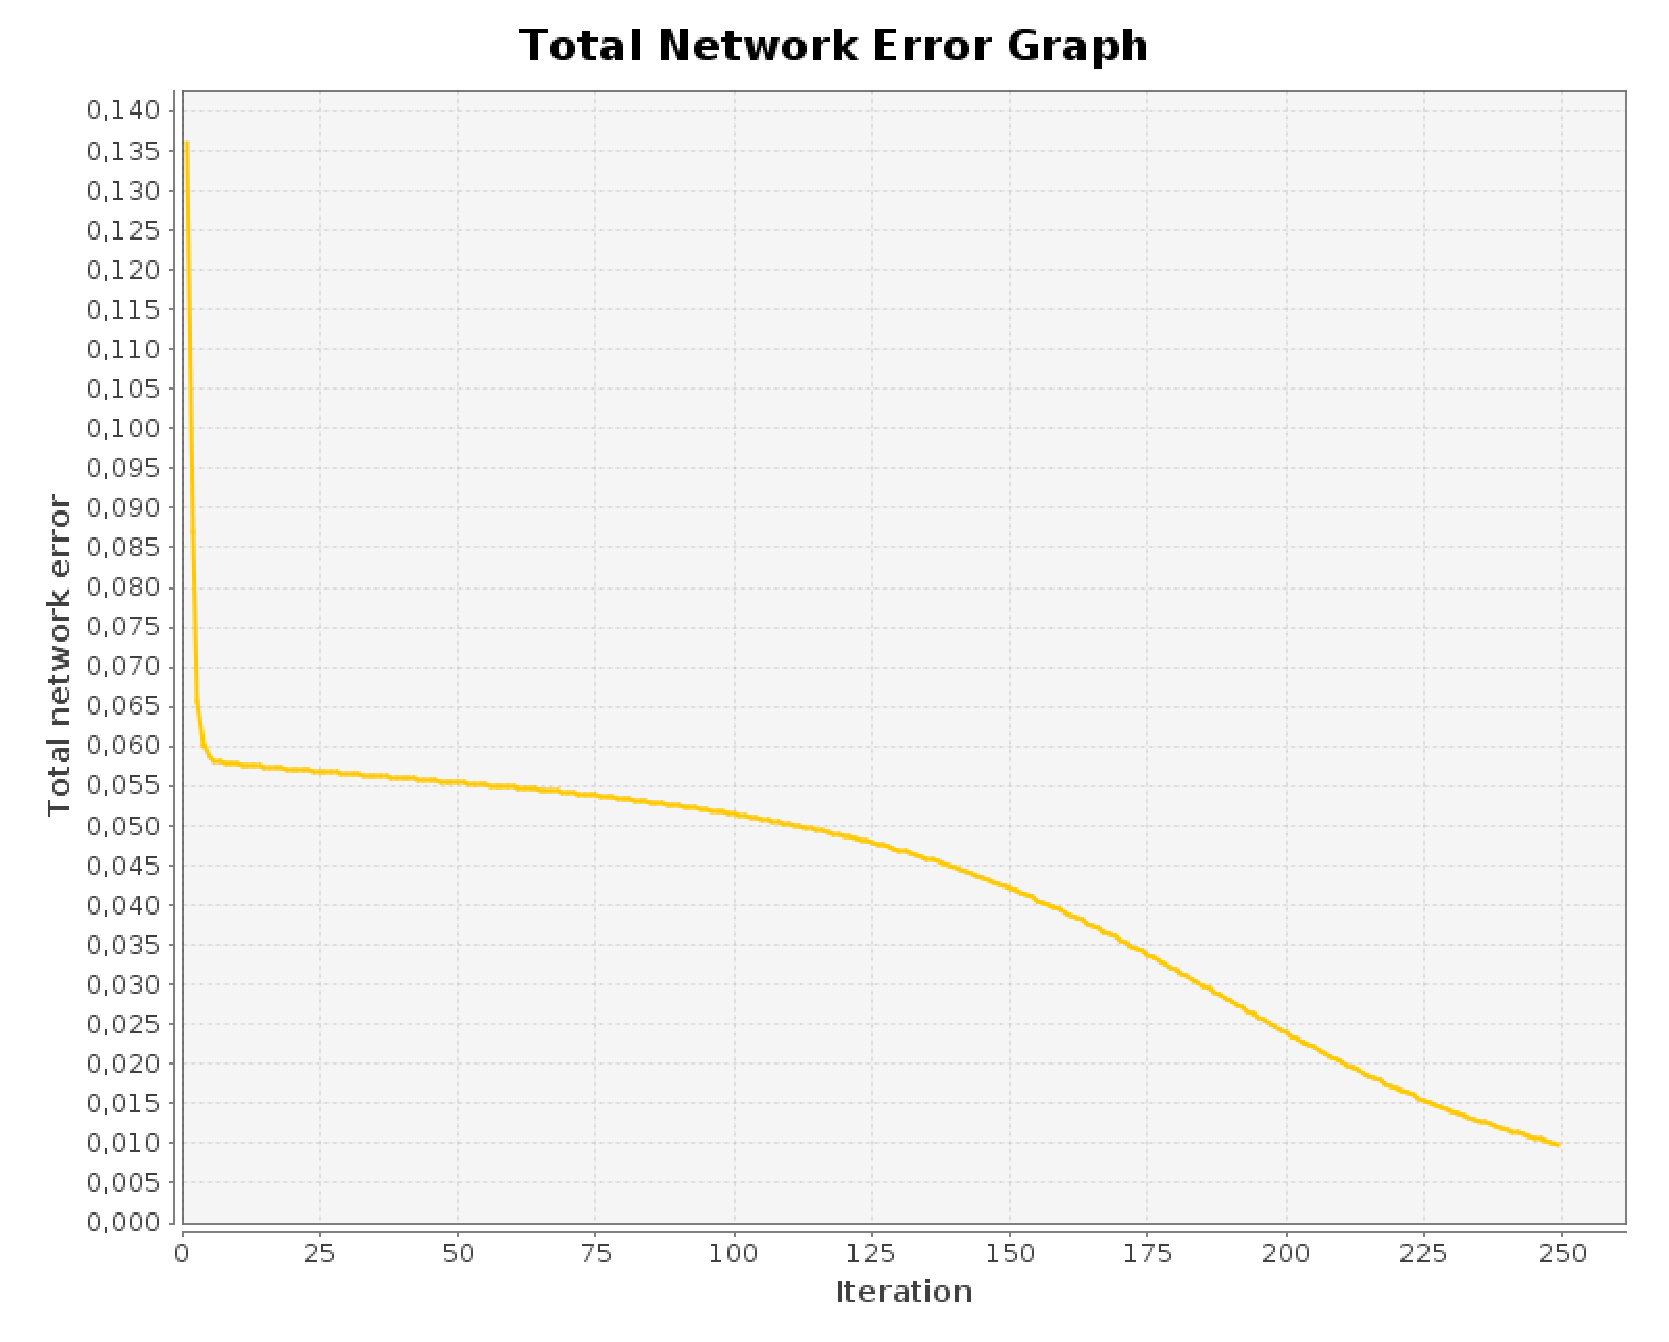
\includegraphics[width=12cm, higth=9cm]{./pics/fct/carre_10_norm_std.eps}


%End content

\addcontentsline{toc}{section}{Références}
\bibliographystyle{plain}
\bibliography{rapport}

\end{document}
